\clearpage
\chapter{Impact of the Battery Capacity on the Optimal Orientation Angle of a PV Cell\label{Chapter_2}}
\settablecounter{3}{1}


Chapter \ref{Chapter_2} will extend the system model in Chapter \ref{Chapter_1} by adding a battery to the BS. The battery is modeled by a Markov chain in this chapter. The system model in Chapter \ref{Chapter_1} has no batteries deployed at the BS. Nonetheless, Chapter \ref{Chapter_1} can be seen as special case of Chapter \ref{Chapter_2} because the batteries can have a battery capacity of $0$ in the system model of Chapter \ref{Chapter_2}.



\section{Literature Review: Batteries at BSs}


It has been shown that the resiliency of cellular networks in disaster events, such as earthquakes and hurricanes, is higher if the energy mix of the cellular networks includes harvest renewable energy instead of relying solely on the power from the main grid \cite{Kwasinski2013LessonsFF}. The service of the cellular network usually breaks down during a disaster event because power lines are damaged and the BSs run out of energy. In addition, back-up generators rely on petrol, which has to be transported to the sites of the BSs via roads, which are often damaged as well in disaster events. Because the cellular network service is so vital during a disaster event to coordinate rescue missions, police operations, and military operations, the cellular network is required to be operational 99.999\% of the time during a year, whereas the power grid is required to be operational only 99.9\% in the U.S. \cite{residential}. In other words, the total yearly outage time of the power grid is less than nine hours, whereas the requirements for cellular networks is much higher than that. Because power grids have lower reliability requirements than that of cellular networks, BSs are typically equipped with batteries that last for a few hours. The capacity of the batteries is usually around four hours but can be higher for some BSs as well \cite{residential}.

PV cells have a very strong diurnal cycle. \cite{CHATTOPADHYAY2017176,RasmussenMortenGrud2012Sabs} showed that a storage capacity of six hours of the average consumption of the appliance is sufficient to smoothen the diurnal cycle of the PV cells. In scenarios where only solar energy is harvested and no other energy sources are available, a storage capacity of twelve hours was recommended by \cite{CHATTOPADHYAY2017176,RasmussenMortenGrud2012Sabs}.


A life cycle energy cost assessment at a stand-alone PV system was conducted in \cite{Thiaux2010602} to evaluate the long term benefits of shifting the energy consumption profile towards the energy generation profile. A better match of both profiles led to a longer battery lifetime due to less battery charging-discharging cycles and the opportunities to downsize the battery capacity and PV cell surface area. 



A good match between the energy generation profile of the PV cell and the energy consumption profile of the BS can be achieved by either installing a small battery (or no battery) with orientation angle optimization or installing a large battery without orientation angle optimization. Nonetheless, batteries are expensive (25 - 250\euro, 220\euro{} and 1500\euro{} per kWh for the battery types Lead-Acid, NaS and Li-Ion, respectively \cite{RUDOLF2013139}) and have a short lifetime (3 - 9 years \cite{CROSSLAND201530}) compared with the warranty lifetimes of PV cells (PV cell manufacturers guarantee a 80\% system performance warranty for around 20 years \cite{6745088}). Therefore, battery replacements significantly contribute to the system lifetime cost \cite{CROSSLAND201530}. Small batteries with orientation angle optimization are practically the more cost-effective option compared with large batteries without orientation angle optimization.


Markov chain models have been used in the literature to model batteries, as seen in \cite{ParzyszFanny2017PCAf, SakrAhmedHamdi2015AoKU,TingwuWang2016ASiS}.


\section{Contributions of Chapter \ref{Chapter_2}}
The contributions of Chapter \ref{Chapter_2} are summarized as follows:

\begin {itemize}

\item Developing a PV cell's orientation angle optimization algorithm with Markov chain based battery model of a solar-powered BS with battery. The algorithm takes into account the battery capacity and the energy consumption profile of the BS. The number of user equipments (UEs) served by the BS throughout the day $\overline{S_{\mathrm{UE}}}(\theta)$ is used as the performance metric to identify the optimal orientation angle.
\item Verifying the accuracy of the proposed algorithm by showing that simulation trials converge based on the law of large numbers to 
the output $\overline{S_{\mathrm{UE}}}(\theta)$ of the proposed algorithm. 
\item Showing that the proposed algorithm (depends on the number of battery states) requires a shorter running time than the simulation trials (depends on the number of trials) for moderate battery state resolutions.
\item Investigating the dependency of the optimal PV cell orientation angle on the given battery capacity.
\end {itemize}

\section{System Model 2 - One PV Cell Powering a BS with Battery\label{system_2}}






Figure  \ref{ene2} depicts the system model 2 considered in this chapter. It consists of an energy generation part with one PV cell, an energy storage part made of a battery, and an energy consumption part composed of a BS. The energy flow follows the arrows in Figure  \ref{ene2} and can only be altered by choosing different orientation angles for the PV cell. All other parameters will be fixed. The energy generation flow is denoted by $G_{\theta,1}(t)$ in Figure \ref{ene2}. The energy consumption flow is divided in a load-independent part, denoted by $c_{\mathrm{con}}$, and a load-dependent part, denoted by $c_\theta(t)$, in Figure \ref{ene2}.

\begin{figure}[H]
	\centering	
		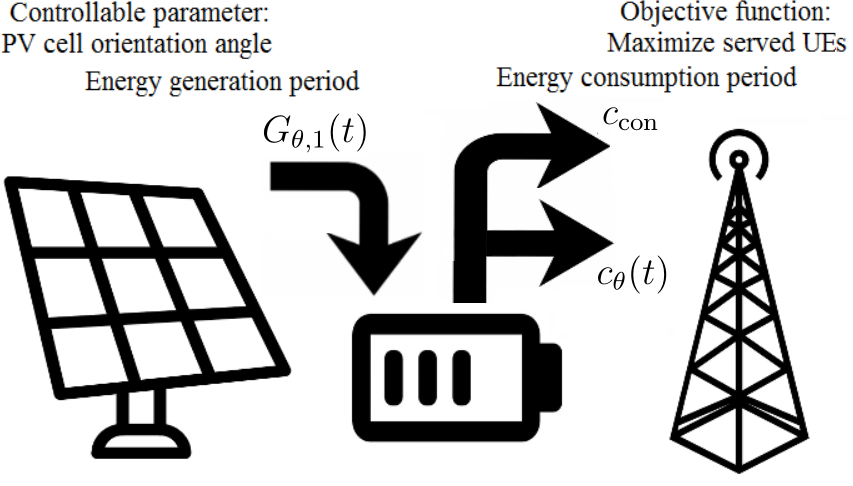
\includegraphics[width=1\columnwidth]{pictures/qq}
\caption{Illustration of system model 2\label{ene2}}
\end{figure}

\subsection{Solar Energy Storage Model}
The BS is only powered by a PV cell. The only controllable parameter in the system model 2 is the PV cell orientation angle. The day is divided into $T$ time steps. The index of a time step is denoted by $t \in \{1,...,T\}$.
Each time step has three distinguish flows, first the energy generation flow will be executed followed by the load-independent energy consumption flow and then the load-dependent energy consumption flow (cf. Figure \ref{ene2}). During the energy generation flow, the amount of generated energy in this time step is calculated and stored in the battery. During the energy consumption flows, the amount of consumed energy by the BS in this time step is subtracted from the battery. In reality all three periods occur simultaneously. For applications that require a simultaneous energy generation and consumption, the length of the time steps can be chosen small enough to achieve a nearly simultaneous energy generation and consumption. 





\subsection{Energy Generation Flow and Load-independent Energy Consumption Flow}\label{energy}


The formula for the normalized energy generated by one PV cell deployed with orientation angle $\theta$ at time step $t$, denoted by $G_{\theta,1}(t)$, has been derived in Chapter \ref{Chapter_1} and can be calculated by (\ref{norma}). 


The battery has an upper bound and a lower bound that determine how much of the generated energy $G_{\theta,1}(t)$ can be stored in the battery. In addition, the load-independent energy consumption of the BS, denoted by $c_{\mathrm{con}}$, has to be subtracted from the battery at the beginning of each time step. 


The available energy, denoted by $a_{\theta}(t)$, in the battery at time step $t$ is as follows:


\begin{equation}\label{available}
a_{\theta}(t)=\max\{0,\min\{b_\theta(t-1)+G_{\theta,1}(t)-c_{\mathrm{con}},b_{\max}\}\},
\end{equation}
\noindent
where $b_{\theta}(t-1)$ is the stored energy in the battery in time step $t-1$, $c_{\mathrm{con}}$ is the load-independent energy consumption of the BS during one time step, and $b_{\max}$ is the maximum battery capacity. The min in (\ref{available}) ensures that the stored energy in the battery is less or equal the maximum battery capacity. The max in (\ref{available}) ensures that the stored energy in the battery is greater or equal $0$. 

The amount of energy stored in the battery at time step $0$ is $b_{\mathrm{begin}}$ as follows:
\begin{equation}
 b_{\theta}(0)=b_{\mathrm{begin}}.
\end{equation}


\subsection{Load-dependent Energy Consumption Flow}\label{traffic}

To model the temporal fluctuation of the BS's energy consumption, the number of user equipments (UEs) connected to the BS at time step $t$ is modeled by a random variable $l(t)$, which follows a Poisson distribution (PD) with density parameter $\lambda(t)$. The number of UEs in the coverage area of a BS is commonly modeled as a Poisson point process in the literature \cite{poisson, baccell00403039, NET-015}. Hence, $l(t)$ is as follows:

\begin{equation}
\label{PPP1}
l(t):=\mathrm{PD}(\lambda(t)).
\end{equation}
Without loss of generality, it is assumed that the BS is located in a business-area. The traffic load profile of a BS in a business-area, denoted by $C_{\mathrm{bus}}(t)$, has been derived in Chapter \ref{Chapter_1} and is given in Figure \ref{all_consumption_profiles}. Nonetheless, the analysis can be applied to any other location and traffic load profile as well.
 Hence, the density parameter $\lambda(t)$ is as follows:

\begin{equation}
\label{P}
\lambda(t)= C_{\mathrm{bus}}(t).
\end{equation}



The number of served UEs\footnote{UEs that cannot be served by the BS due to a lack of renewable stored energy in the battery might be off-loaded to other BSs or the BS uses main grid energy to serve these UEs. Only UEs which are served by the available renewable energy will be counted by $s_\theta(t)$.} by the BS at time step $t$, denoted by $s_\theta(t)$, is limited either by the number of UEs connected to the BS or the available energy as follows:


\begin{equation}
\label{PPP2}
s_\theta(t)=\min\Big\{l(t),\Big\lfloor \frac{a_\theta(t)}{c_{\mathrm{UE}}}\Big\rfloor\Big\},
\end{equation}



\noindent
where $a_{\theta}(t)$ is the available energy at time step $t$, and $c_{\mathrm{UE}}$ is the average amount of energy needed to serve one UE.

The load-dependent energy consumption $c_\theta(t)$ of the BS in time step $t$ is given by


\begin{equation}
\label{PPP3}
c_\theta(t)=s_\theta(t)\cdot c_{\mathrm{UE}}.
\end{equation}



 The residual energy in the battery at the end of time step $t$ can be calculated by

\begin{equation}
\label{bat}
b_\theta(t)=a_\theta(t)-c_\theta(t).
\end{equation}

\subsection{Determination of the Average Number of Served UEs}
Eq. (\ref{PPP2}) ensures that the consumed energy by the BS is less than or equal to the stored energy in the battery. As a result, it is possible that some UEs cannot be served\footnote{UEs that cannot be served by the BS due to a lack of renewable stored energy might be off-loaded to other BSs or the BS uses main grid energy to serve these UEs. Only UEs which are served by the available renewable stored energy will be counted by $s_\theta(t)$.} by the BS due to a lack of renewable stored energy. Therefore, the number of served UEs $S_{\mathrm{UE}}(\theta)$ throughout the day by a PV cell with orientation angle $\theta$ is used as the performance metric, where $S_{\mathrm{UE}}(\theta)$ is as follows:

\begin{equation}
\label{PPP}
S_{\mathrm{UE}}(\theta)=\sum_{t=1}^{T} s_\theta(t).
\end{equation}

Because the $l(t)$ values are random variables, $\overline{S_{\mathrm{UE}}}(\theta)$ denotes the average value of $S_{\mathrm{UE}}(\theta)$.



The orientation angle $\theta$ which achieves the highest $\overline{S_{\mathrm{UE}}}(\theta)$ value is considered as optimal orientation angle $\theta^*$ as follows:

\begin{equation}
\label{sol}
\theta^* =\mathrm{arg} \enskip \mathrm{max}_{\theta} \enskip\overline{S_{\mathrm{UE}}}(\theta).
\end{equation}





\section{Orientation Angle Optimization Algorithm with Markov Chain Based Battery\label{jj}}
The following PV cell's orientation angle optimization algorithm with Markov chain based battery model (Algorithm \ref{mar}) can efficiently determine the optimal orientation angle of the PV cell at a BS with battery. To show the effectiveness of the proposed algorithm, a simulation algorithm (Algorithm \ref{sim}) will be developed in the Section \ref{see} as well. The advantages of the proposed algorithm in comparison with the simulation algorithm (Algorithm \ref{sim}) with respect to accuracy and running time will be evaluated in Section \ref{results_system_2}.

All energy values are discretized with a precision of $\mu$, i.e., $\tilde{G}_{\theta,1}(t)$ will be the closest multiple of $\mu$ from $G_{\theta,1}(t)$. For example, if $\mu=\frac{1}{1000}$, and $G_{\theta,1}(t)=1.2756$, then $\tilde{G}_{\theta,1}(t)=1.276$.


There are $S_{\mathrm{max}}=\frac{b_{\max}}{\mu}+1$ battery energy states. The battery energy states $0, 1, 2, 3, ...,$ and $\frac{b_{\max}}{\mu}$ represent $0, \mu, 2\cdot\mu, 3\cdot\mu, ...,$ and $b_{\max}$ units of normalized energy, respectively. Without loss of generality, $b_{\mathrm{begin}}$, $b_{\max}$, $c_{\mathrm{UE}}$, and $c_{\mathrm{con}}$ are multiple of $\mu$.

 The expression $\mathbb{P}(a_{\theta}(t)=i)=x$ means that the probability of having $i$ units of normalized energy available in the battery at the beginning of time step $t$ is $x$. The expression $\mathbb{P}(b_{\theta}(t)=i)=x$ means that the probability of the battery having stored $i$ units of normalized energy at the end of time step $t$ is $x$.


The following subsections will go through the Algorithm \ref{mar} line by line. The expression $\lfloor x \rfloor$ means that the variable $x$ is rounded down to the nearest integer value.


\subsection{Markov Chain Initialization\label{Tet}}



Because $l(t)$ is a Poisson distributed random variable, $\mathbb{P}(l(t)= r)$, and $\mathbb{P}(l(t)\geq r)$ are $\frac{\lambda(t)^r \cdot e^{-\lambda(t)}}{r!}$, and $1 - \sum_{w=0}^{r-1}\frac{\lambda(t)^w\cdot e^{-\lambda(t)}}{w!}$, respectively \cite{poisson_formula} (Algorithm \ref{mar} line: \ref{in1} - \ref{in2}). 

$S_{\mathrm{max}}$ is initialized (Algorithm \ref{mar} line: \ref{battery_stages}).
The initial battery state $b_\theta(0)$ is equal to $b_{\mathrm{begin}}$ at the beginning of Algorithm \ref{mar}. Therefore, the probability of the battery state being $b_{\mathrm{begin}}$ at time step $0$ is $1$, whereas all the other battery states have a probability of $0$ (Algorithm \ref{mar} line: \ref{ini1_mar} - \ref{ini2_mar}). There are no UEs served at the beginning of Algorithm \ref{mar} (Algorithm \ref{mar} line: \ref{sss}).
Eq. (\ref{P}) is used to calculate the UE density parameters $\lambda(t)$ for all time steps (Algorithm \ref{mar} line: \ref{c_mar}). 

\subsection{Energy Generation Flow and Load-independent Energy Consumption Flow of Algorithm \ref{mar}}

All $\mathbb{P}(a_\theta(t)=i)$ values are set at $0$ at the beginning (Algorithm \ref{mar} line: \ref{a_ini}).
If the battery is in state $i$, $S_{\mathrm{Shift}}$ calculates the new battery state after the generated energy $\tilde{G}_{\theta,1}(t)$ is added to the battery and the load-independent energy consumption of the BS $c_{\mathrm{con}}$ is subtracted from the battery (Algorithm \ref{mar} line: \ref{she}). $S_{\mathrm{Shift}}$ takes into account the upper bound and the lower bound of the battery (Algorithm \ref{mar} line: \ref{she}).
If $\tilde{G}_{\theta,1}(t)>c_{\mathrm{con}}$, then every battery state increases by $\frac{\tilde{G}_{\theta,1}(t)-c_{\mathrm{con}}}{\mu}$ battery states or reaches the maximum battery state $S_{\mathrm{max}}-1$ if it comes to a battery overflow. This is depicted in Figure \ref{fig:gener}.
If $\tilde{G}_{\theta,1}(t)<c_{\mathrm{con}}$, then every battery state decreases by $\frac{c_{\mathrm{con}}-\tilde{G}_{\theta,1}(t)}{\mu}$ battery states or reaches the minimum battery state $0$ if the battery depletes. This is depicted in Figure \ref{fig:gener2}.
If $\tilde{G}_{\theta,1}(t)=c_{\mathrm{con}}$, there is no energy added or subtracted from the battery.
Each transition occurs with a probability of $1$, which is depicted on top of each arrow in Figures \ref{fig:gener} - \ref{fig:gener2}.

The probability of the battery state being $i$ at the time step $t-1$, i.e., $\mathbb{P}(b_\theta(t-1)=i)$, is added to the probability of the new battery state, i.e., $\mathbb{P}(a_\theta(t)=S_{\mathrm{Shift}})$ (Algorithm \ref{mar} line: \ref{shift}).






\begin{figure}[H]
	\centering
		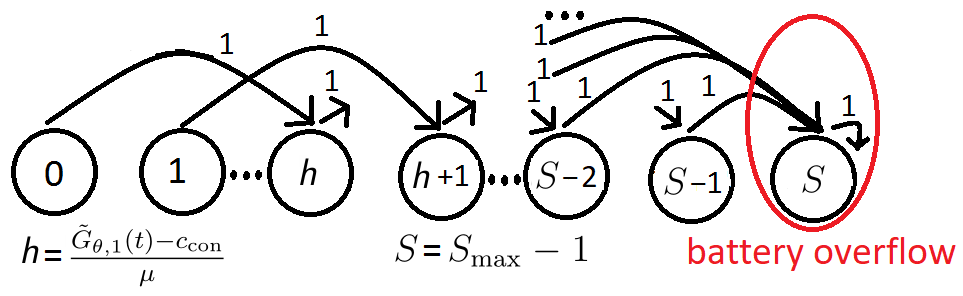
\includegraphics[scale=0.6]{pictures/1}
	\caption{Energy generation flow and load-independent energy consumption flow if $\tilde{G}_{\theta,1}(t)>c_{\mathrm{con}}$\label{fig:gener}}
\end{figure}

\begin{figure}[H]
	\centering
		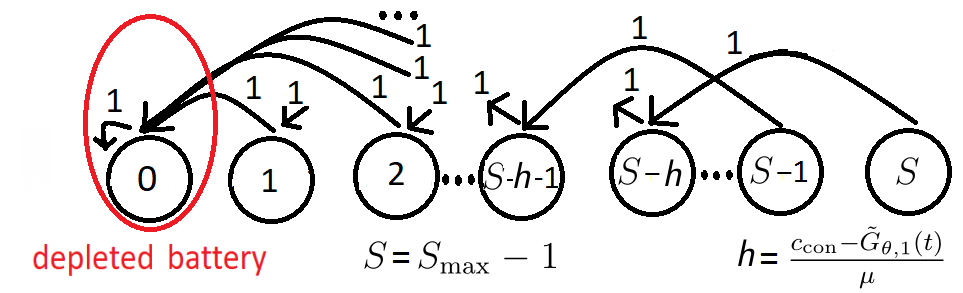
\includegraphics[scale=0.6]{pictures/EN}
	\caption{Energy generation flow and load-independent energy consumption flow if $\tilde{G}_{\theta,1}(t)<c_{\mathrm{con}}$\label{fig:gener2}}
\end{figure}




\subsection{Load-dependent Energy Consumption Flow of Algorithm \ref{mar}}
The number of UEs in the coverage area of the BS, denoted by $l(t)$, is Poisson distributed with density parameter $\lambda(t)$, i.e., $l(t):= \mathrm{PD}(\lambda(t))$. The probability of $l(t)$ to be equal to an integer value $r$, denoted by $\mathbb{P}(l(t)=r)$, is given for a Poisson distribution by $\frac{\lambda(t)^r \cdot e^{-\lambda(t)}}{r!}$ \cite{poisson_formula} (Algorithm \ref{mar} line: \ref{in1}). The expression $\mathbb{P}(l(t)\geq r)$ is given for a Poisson distribution by $1 - \sum_{w=0}^{r-1}\frac{\lambda(t)^w\cdot e^{-\lambda(t)}}{w!}$ \cite{poisson_formula} (Algorithm \ref{mar} line: \ref{in2}).

Each served UE consumes $c_{\mathrm{UE}}$ units of normalized energy in each time step. Therefore, every battery state has to be decreased by $\frac{c_{\mathrm{UE}}}{\mu}$ battery states for every served UE in each time step.

This paragraph derives the update formulas for the battery states from $\frac{c_{\mathrm{UE}}}{\mu}$ to $S_{\max}-1$ (Algorithm \ref{mar} line: \ref{c11} - \ref{c12}). Figure \ref{fig:consum1} shows only the incoming arrows for the battery state $\frac{c_{\mathrm{UE}}}{\mu}$ as an example. The battery state $i \in \{\frac{c_{\mathrm{UE}}}{\mu},...,S_{\max}-1\}$ has $\Big\lfloor \frac{(S_{\max}-1-i)\cdot\mu}{c_{\mathrm{UE}}} \Big\rfloor + 1 $ incoming arrows. $r \in \big\{0,...,\Big\lfloor\frac{(S_{\max}-1-i)\cdot\mu}{c_{\mathrm{UE}}}\Big\rfloor\big\}$ describes the transition from battery state $i+r \cdot \frac{c_{\mathrm{UE}}}{\mu}$ to battery state $i$ when exactly $r$ UEs are served. The transition probability is $\mathbb{P}(l(t)=r) $ for this transition which is depicted next to the transition arrow in Figure \ref{fig:consum1}.

This paragraph derives the update formulas for the battery states from $0$ to $\frac{c_{\mathrm{UE}}}{\mu}-1$ (Algorithm \ref{mar} line: \ref{c21} - \ref{c22}). Figure \ref{fig:consum2} shows only the incoming arrows for the battery state $0$ as an example. The battery state $i \in \{0,...,\frac{c_{\mathrm{UE}}}{\mu}-1\}$ has $\Big\lfloor \frac{(S_{\max}-1-i)\cdot\mu}{c_{\mathrm{UE}}} \Big\rfloor + 1 $ incoming arrows. $r \in \big\{0,...,\Big\lfloor \frac{(S_{\max}-1-i)\cdot\mu}{c_{\mathrm{UE}}} \Big\rfloor\big\}$ describes the transition from battery state $i+r \cdot \frac{c_{\mathrm{UE}}}{\mu}$ to battery state $i$ when more than $r-1$ UEs are in the coverage area of the BS, which means the BS can only serve $r$ UEs and the remaining UEs cannot be served due to the lack of available renewable stored energy. The transition probability is $\mathbb{P}(l(t)\geq r) $ for this transition which is depicted next to the transition arrow in Figure \ref{fig:consum2}.



\begin{figure}[H]
	\centering
		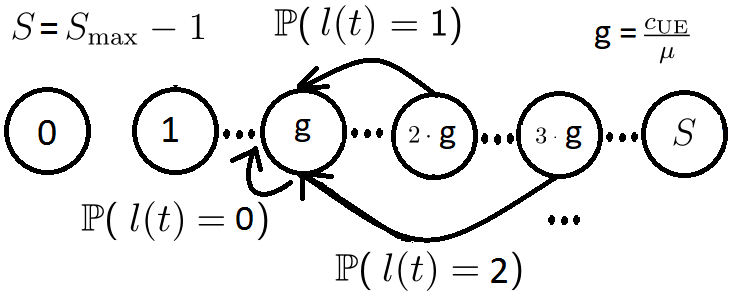
\includegraphics[scale=0.6]{pictures/33}
	\caption{Energy consumption flow for the battery state $\frac{c_{\mathrm{UE}}}{\mu}$ \label{fig:consum1}}
\end{figure}


\begin{figure}[H]
	\centering
		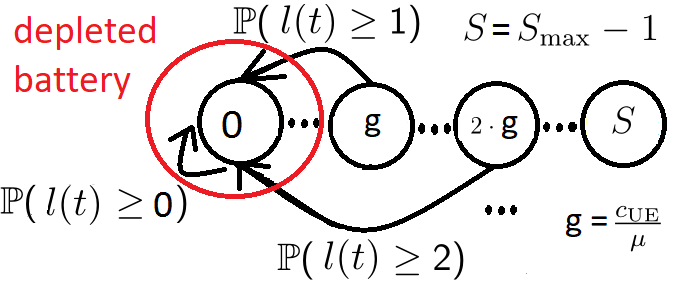
\includegraphics[scale=0.6]{pictures/rr}
	\caption{Energy consumption flow for the battery state $0$ \label{fig:consum2}}
\end{figure}


\subsection{Determination of the Average Number of Served UEs of Algorithm \ref{mar}}
When the battery is in state $i$, it can serve $r \in \{0,...,\Big\lfloor \frac{i\cdot\mu}{c_{\mathrm{UE}}} \Big\rfloor\}$ UEs. When $r\in\{0,...,\Big\lfloor \frac{i\cdot\mu}{c_{\mathrm{UE}}} \Big\rfloor   -1\}$, the energy in the battery is decreased from battery state $i$ with the transition probability of $\mathbb{P}(l(t)=r)$. Exactly $r$ UEs were served, that is why the expression in Algorithm \ref{mar} line: \ref{hi1} is multiplied by $r$. When $r= \Big\lfloor \frac{i\cdot\mu}{c_{\mathrm{UE}}} \Big\rfloor$, the energy in the battery is decreased from battery state $i$ with the transition probability of $\mathbb{P}(l(t)\geq \Big\lfloor \frac{i\cdot\mu}{c_{\mathrm{UE}}} \Big\rfloor) $. Exactly $\Big\lfloor \frac{i\cdot\mu}{c_{\mathrm{UE}}} \Big\rfloor$ UEs were served, that is why the expression in Algorithm \ref{mar} line: \ref{hi2} is multiplied by $\Big\lfloor \frac{i\cdot\mu}{c_{\mathrm{UE}}} \Big\rfloor$. 



The PV cell's orientation angle optimization algorithm with Markov chain based battery model is summarized as follows:


\begin{breakablealgorithm}                
\caption{\textbf{Algorithm 1: } PV cell's orientation angle optimization algorithm with Markov chain based battery model\label{mar}}   \singlespacing                       
\begin{algorithmic} [1]                 
    \Require $\gamma$, $\mu$, $T$, $b_{\mathrm{begin}}$, $b_{\max}$, $c_{\mathrm{con}}$, $c_{\mathrm{UE}}$, $\tilde{G}_{\theta,1}(t) \enskip \forall t\enskip\forall \theta  \text{, and } C_{\mathrm{bus}}(t) \enskip \forall t$  
   \Ensure $\theta^*$
	\State \% $\mathbb{P}(l(t)=r)=\frac{\lambda(t)^r \cdot e^{-\lambda(t)}}{r!}$ \label{in1}
	\State \% $\mathbb{P}(l(t)\geq r)=1 - \sum_{w=0}^{r-1}\frac{\lambda(t)^w\cdot e^{-\lambda(t)}}{w!}$ \label{in2}
	\item[]
	\For{all $\theta\in \{-40^{\mathrm{o}},-35^{\mathrm{o}},...,90^{\mathrm{o}}\}$}
	\item[]
	\State \text{ \% Initialization} \label{ini1} 		
	\State $S_{\mathrm{max}}=\frac{b_{\max}}{\mu}+1$\label{battery_stages}
		\State $\mathbb{P}(b_\theta(0)=\frac{b_{\mathrm{begin}}}{ \mu})=1$ \label{ini1_mar}
\State $\mathbb{P}(b_\theta(0)=i)=0 \quad \quad \quad \forall i \in \{0,...,S_{\mathrm{max}}-1\} \setminus  (\frac{b_{\mathrm{begin}}}{ \mu})$ \label{ini2_mar}
\State $\overline{S_{\mathrm{UE}}}(\theta)=0$\label{sss}
	\For{$t=1:T$}
		\State $\lambda(t)=C_{\mathrm{bus}}(t) $\label{c_mar}
	\EndFor
		\item[]

		
\For{$t=1:T$}
		\State \text{ \% Energy generation flow and load-independent energy consumption flow}\label{gen1}  
		
	\State $\mathbb{P}(a_\theta(t)=i)=0\quad \quad \quad\quad \quad \forall i \in \{0,...,S_{\mathrm{max}}-1\}\quad$ \text{ \% Initialization}\label{a_ini}
		\For{$i \in \{0,...,S_{\mathrm{max}}-1\}$}
		
		\State $S_{\mathrm{Shift}}=\max\{0,\min\{i+\frac{\tilde{G}_{\theta,1}(t)-c_{\mathrm{con}}}{\mu},\frac{b_{\mathrm{max}}}{\mu}\}\}$\label{she}
		\State $\mathbb{P}(a_\theta(t)=S_{\mathrm{Shift}})=\mathbb{P}(a_\theta(t)=S_{\mathrm{Shift}})+\mathbb{P}(b_\theta(t-1)=i)$\label{shift}
		\EndFor
		
		\item[]
		\State \text{ \% Adding the average number of UEs served at time step $t$ to $\overline{S_{\mathrm{UE}}}(\theta)$}
    \For {$i=0:S_{\mathrm{max}}-1$}
     \For {$r=0: \lfloor \frac{i\cdot \mu}{c_{\mathrm{UE}}} \rfloor   -1$}
    \State $\overline{S_{\mathrm{UE}}}(\theta)=\overline{S_{\mathrm{UE}}}(\theta)+ r \cdot \mathbb{P}(l(t)=r) \cdot \mathbb{P}(a_\theta(t)=i) $ \label{hi1}
       \EndFor
   \State      $\overline{S_{\mathrm{UE}}}(\theta)=\overline{S_{\mathrm{UE}}}(\theta)+ \lfloor \frac{i \cdot \mu}{c_{\mathrm{UE}}} \rfloor \cdot \mathbb{P}(l(t)\geq \lfloor \frac{i\cdot \mu}{c_{\mathrm{UE}}} \rfloor ) \cdot \mathbb{P}(a_\theta(t)=i) $\label{hi2}   
       \EndFor 
		\item[]
			\State \text{ \% Load-dependent energy consumption flow} \label{con1} 
			\State $\mathbb{P}(b_\theta(t)=i)=\sum_{r=0}^{ \Big\lfloor \frac{(S_{\mathrm{max}}-1-i)\cdot \mu}{c_{\mathrm{UE}}} \Big\rfloor } \Big(  \mathbb{P}(l(t)\geq r) \cdot \mathbb{P}(a_\theta(t)=i +r \cdot \frac{c_{\mathrm{UE}}}{\mu})\Big) $\label{c21}  
			
		\State $	\quad \forall i \in \{0,...,\frac{c_{\mathrm{UE}}}{\mu}-1\}$ \label{c22}  
    \State $\mathbb{P}(b_\theta(t)=i)=\sum_{r=0}^{ \Big\lfloor \frac{(S_{\mathrm{max}}-1-i)\cdot \mu}{c_{\mathrm{UE}}} \Big\rfloor }  \Big( \mathbb{P}(l(t)=r)  \cdot\mathbb{P}(a_\theta(t)=i +r \cdot \frac{c_{\mathrm{UE}}}{\mu})\Big)$\label{c11}  
	\State 	$\quad \enskip\!\! \forall i \in \{\frac{c_{\mathrm{UE}}}{\mu},...,S_{\mathrm{max}}-1\}$ \label{c12}  
\EndFor
\EndFor
\Return $\theta^*=\arg \displaystyle\max_{\theta\in[-90^{\mathrm{o}},90^{\mathrm{o}}]} \overline{S_{\mathrm{UE}}}(\theta)$
\end{algorithmic}
\end{breakablealgorithm}




\section{Derivation of a Simulation Algorithm as Baseline \label{see}}

Eqs. (\ref{available}) - (\ref{sol}) are used to derive the following simulation algorithm (Algorithm \ref{sim}). Algorithm \ref{sim} is the baseline for the performance comparison with the shown proposed algorithm (Algorithm \ref{mar}).


 



\begin{algorithm} [H]                     
\caption{Simulation algorithm\label{sim}}     
\label{alg2}                    
\begin{algorithmic} [1] 
          
    \Require $\gamma$, $L$, $T$, $b_{\mathrm{begin}}$, $b_{\max}$, $c_{\mathrm{con}}$, $c_{\mathrm{UE}}$, $G_{\theta,1}(t) \enskip \forall t\enskip\forall \theta  \text{, and } C_{\mathrm{bus}}(t) \enskip \forall t$  
   \Ensure $\theta^*$
		\For{all $\theta\in \{-40^{\mathrm{o}},-35^{\mathrm{o}},...,90^{\mathrm{o}}\}$}
	\item[]
	   \State  $\overline{S_{\mathrm{UE}}}(\theta)=0$
				\For{$l=1:L$}
				\item[]
					\State \text{\% Initialization} 
\State $b_\theta(0)=b_{\mathrm{begin}}\quad$
		\For{$t=1:T$}
							\State \text{\% Energy generation flow}
        \State $a_\theta(t)=\max\{0,\min\{b_\theta(t-1)+G_{\theta,1}(t)-c_{\mathrm{con}},b_{\max}\}\}$ \label{h_sim}
			\item[]
			\State \text{\% Energy consumption flow} 
			\State $\lambda(t)=C_{\mathrm{bus}}(t)$  \label{c_sim}
			\State	$s_\theta(t)=\min\{\mathrm{PD}(\lambda(t)),\lfloor \frac{a_\theta(t)}{c_{\mathrm{UE}}}\rfloor\}$,
	\State $b_\theta(t)=a_\theta(t)-s_\theta(t)\cdot c_{\mathrm{UE}}$ 
		\EndFor
		

		\State $\overline{S_{\mathrm{UE}}}(\theta)=\overline{S_{\mathrm{UE}}}(\theta)+\sum_{t=1}^{T} s_\theta(t)$
		\EndFor 			 
\State $\overline{S_{\mathrm{UE}}}(\theta)= \overline{S_{\mathrm{UE}}}(\theta)/L$
\EndFor
		\Return $\theta^*=\arg \displaystyle\max_{\theta\in[-90^{\mathrm{o}},90^{\mathrm{o}}]} \overline{S_{\mathrm{UE}}}(\theta)$
\end{algorithmic}
\end{algorithm}


The simulation algorithm (Algorithm \ref{sim}) has to be run for a large number $L$ until the average of the $S_{\mathrm{UE}}(\theta)$ value converges to a fixed value, denoted by $\overline{S_{\mathrm{UE}}}(\theta)$. 

\section{Results and Discussion\label{results_system_2}}



\subsection{Running Time of the proposed Algorithm and the Simulation Algorithm\label{n}}
The simulation algorithm has a running time of $\mathcal{O}(L \cdot T)$, whereas the proposed algorithm has a running time of $\mathcal{O}(S_{\max}^2 \cdot T)$. Therefore, the proposed algorithm outperforms the simulation algorithm when the battery is not divided into too many battery states $S_{\max}$. Especially for small BSs with small battery capacities, the proposed algorithm is an effective tool to determine the optimal PV cell orientation. 


\subsection{Accuracy of the Proposed Algorithm and the Simulation Algorithm \label{anna}}
The proposed algorithm has the advantage that it can generate the exact $\overline{S_{\mathrm{UE}}}(\theta)$ value, whereas the simulation algorithm only converges to the $\overline{S_{\mathrm{UE}}}(\theta)$ value.
The parameters in Table \ref{frog} are used for the simulation algorithm and the proposed algorithm. Both algorithms are run for every orientation angle $\theta \in \{-40^{\mathrm{o}},-35^{\mathrm{o}},...,85^{\mathrm{o}},90^{\mathrm{o}}\}$ with constant inclination angle $\gamma=36^{\mathrm{o}}$ (optimal inclination angle for Greenwich (London, UK) in summer). The simulation algorithm is run $L=100000$ times to achieve a good convergence. 





\begin{longtable}{@{}l*{2}{|l}l@{}}
\caption{\\ Input parameters of system model 2\label{frog}}\\ \toprule
\textbf{Parameter}	&\textbf{Description}				&  \textbf{Value} \\ \midrule
$\theta$  & Orientation angle of PV cell&$\in \{-40^{\mathrm{o}},-35^{\mathrm{o}},...,90^{\mathrm{o}}\}$  \\
$\theta^*$  & Optimal orientation angle of PV cell&$\in \{-40^{\mathrm{o}},-35^{\mathrm{o}},...,90^{\mathrm{o}}\}$  \\
$\gamma$ & Inclination angle of PV cell& $36^{\mathrm{o}}$ \\
$\lambda(t)$ &Density parameter of Poisson &  \\
&distributed random variable at time step $t$& Eq. (\ref{P}) \\
$\mu$ & Precision of the discretization &  \\
 &of the energy values/ battery states& $\frac{1}{1000}$ \\
$C_{\mathrm{bus}}(t)$ & Business-area traffic load profile at time step $t$& Figure \ref{all_consumption_profiles}\\
$G_{\theta,1}(t)$ &Normalized energy generated by&\\
& one PV cell installed with $\theta$ at time step $t$&Eq. (\ref{norma})\\
$\tilde{G}_{\theta,1}(t)$ &Closest multiple of $\mu$ from $G_{\theta,1}(t)$&\\
$L$  &Number of loops in simulation algorithm&$100000$\\
$S_{\mathrm{Shift}}$  &New battery state after $\tilde{G}_{\theta,1}(t)$ is added 
&\\
 &and $c_{\mathrm{con}}$ is subtracted
&(Algorithm \ref{mar} line: \ref{she})\\
$S_{\max}$&Number of battery energy states& $\frac{b_{\max}}{\mu}+1$ \\
$S_{\mathrm{UE}}(\theta)$ &Number of served  &\\
 & UEs throughout the day &Eq. (\ref{PPP})\\
$\overline{S_{\mathrm{UE}}}(\theta)$ &Average number of served  &\\
 &UEs throughout the day &Eq. (\ref{PPP})\\
$T$ &Number of time steps&96\\
$a_\theta(t)$&Available energy in the battery &\\
&at the beginning of time step $t$&Eq. (\ref{available})\\
$b_\theta(t)$&Stored energy in the battery &\\
&at the end of time step $t$&Eq. (\ref{bat})\\
$b_{\mathrm{begin}}$&Amount of energy stored&\\
& in the battery at time step $0$&$0$ \\
$b_{\max}$  &Battery capacity& $\in\{1,3,10\}$\\
$c_\theta(t)$&Load-dependent energy consumption &\\
& of the BS at time step $t$&Eq. (\ref{PPP3})\\
$c_{\mathrm{con}}$ &Load-independent energy consumption& \\
 &of the BS in one time step & $0.5$\\
$c_{\mathrm{UE}}$ &Average amount of energy & \\
 & needed to serve one UE & $0.2$\\
$d$ &Day of the year &165 (June)\\
$lat$ &Latitude  &$51.4767^{\mathrm{o}}$ North \\
& & (Greenwich)\\
$lon$ &Longitude &$0.0003^{\mathrm{o}}$ West \\
& & (Greenwich)\\
$l(t)$&Number of UEs connected  &\\
&to the BS at time step $t$ &Eq. (\ref{PPP1})\\
$s_\theta(t)$&Number of served UEs at time step $t$&Eq. (\ref{PPP2})\\
\bottomrule
\end{longtable}







Figure \ref{result1} compares the simulation algorithm and the proposed algorithm. It shows that the simulation algorithm and the proposed algorithm calculate the same $\overline{S_{\mathrm{UE}}}(\theta)$ value for each orientation angle $\theta$ ($L=100000$). Therefore, the proposed algorithm accurate describes the limit of the simulation algorithm convergence. 

\begin{figure}[H]
	\centering
		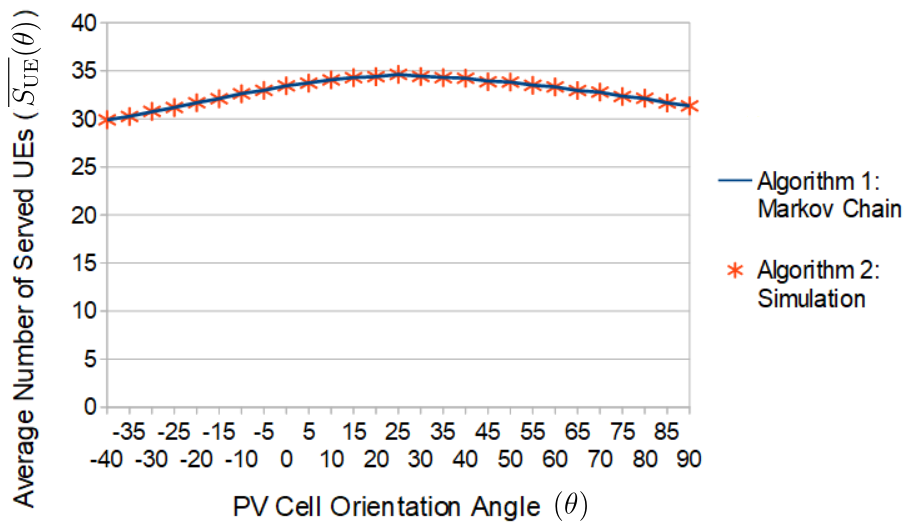
\includegraphics[width=1\textwidth]{pictures/sim_vs_markov}
\caption{Comparison between the proposed algorithm and the simulation algorithm. $b_{\max}$ was set at 3. \label{result1}}
\end{figure}


\subsection{Dependency of the Optimal PV Cell Orientation Angle on the Given Battery Capacity\label{new}}


 


Figure \ref{result2} plots the average number of served UEs $\overline{S_{\mathrm{UE}}}(\theta)$ versus the PV cell orientation angle $\theta$ for the three battery capacities: $b_{\mathrm{max}}=1, 3,$ and $10$. Figure \ref{result2} shows that not only the given energy generation and consumption profile is important for the outcome of the optimization but also the battery capacity. 

If the battery capacity is small, i.e., $b_{\max}=1$, a lot of energy is wasted in the morning and midday hours, whereas UEs cannot be served in the afternoon due to a lack of available renewable stored energy in the battery. Therefore, PV cells orientated to the west between $25^{\mathrm{o}}$ to $40^{\mathrm{o}}$ outperform the other orientation angles because west-orientated PV cells shift the energy generation towards the load profile. 

If the battery capacity is large, i.e., $b_{\max}=10$, less energy is wasted in the morning and midday hours due to the larger battery capacity. Therefore, the optimal orientation angle is $\theta^*=0^{\mathrm{o}}$ and the PV cell should be oriented towards the south. South-oriented PV cells generate the most energy throughout the day among all possible orientation angles.

If the battery capacity is moderate, i.e., $b_{\max}=3$, the optimal orientation angle is between the optimal orientation angles of the other two cases.






\begin{figure}[H]
	\centering
		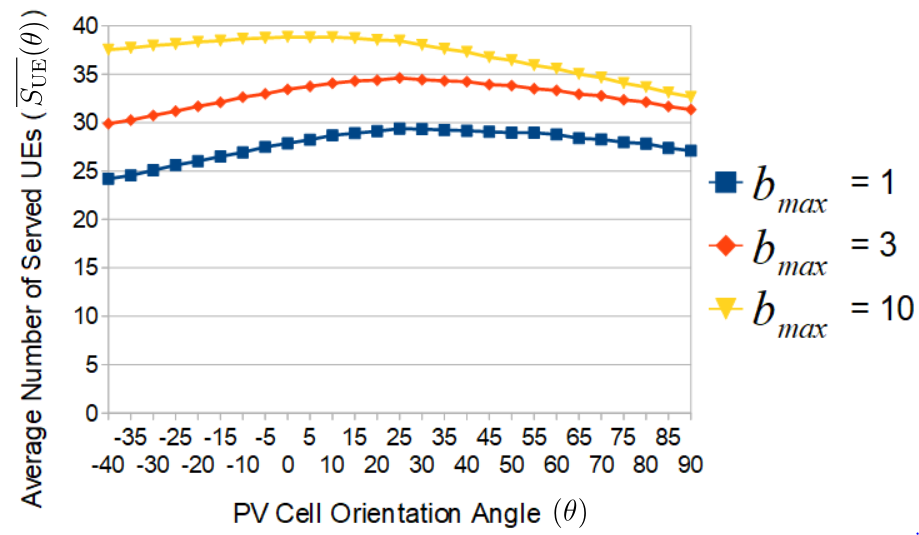
\includegraphics[width=1\textwidth]{pictures/different_batteries}
\caption{Average number of served UEs per day $\overline{S_{\mathrm{UE}}}(\theta)$ vs. PV cell orientation angle $\theta$ for different battery capacities $b_{\mathrm{max}}$ \label{result2}}
\end{figure}

\section{Summary of Chapter \ref{Chapter_2}\label{sum_Chapter_2}}

In Chapter \ref{Chapter_2}, a battery model was added to the system model. The battery model is based on a Markov chain. The proposed PV cell's orientation angle optimization algorithm with Markov chain based battery model has a running time dependent on the squared number of energy states of the battery $S_{\max}$ and the time resolution $T$. The number of UEs served by the BS throughout the day $\overline{S_{\mathrm{UE}}}(\theta)$ was used as the performance metric to identify the optimal orientation angle. The accuracy of the proposed algorithm was verified by showing that simulation trials converge based on the law of large numbers to the output $\overline{S_{\mathrm{UE}}}(\theta)$ of the proposed algorithm. 
The effects of different battery capacities on the optimal PV cell orientation angle were investigated. 
Whereas BSs with small battery capacities significantly improved their performance by orientation angle optimization, BSs with large battery capacities should orient the PV cells towards the south. The importance of the PV cell orientation angle optimization was verified for a BS with small battery capacity $b_{\max}=1$ located in a business-area in Greenwich (London, UK) in summer. Also PV cells are normally orientated to the south in Greenwich (London, UK), the algorithm revealed that the optimal orientation angle is between $25^{\mathrm{o}}$ to $40 ^{\mathrm{o}}$ to the west. 




